\chapter[Simulado 4]{Simulado}

\num{1} O número $\sqrt{12}$ é um número:

\begin{escolha}

\item
  Natural
\item
  Inteiro
\item
  Racional
\item
  Irracional
\end{escolha}


\num{2} A luz viaja 9,45\cdot10\textsuperscript{15} metros por ano. O ano tem 3,15\cdot10\textsuperscript{7} segundos.

Para determinar a velocidade calculamos a razão entre a distância e o
tempo.

Qual a velocidade da luz, em m/s?

\begin{escolha}
\item
  $3 \cdot 10^{8}$
\item
  $9,45 \cdot 10^{15}$
\item
  $3,15 \cdot 10^{7}$
\item
  $6,3 \cdot 10^{8}$
\end{escolha}

\num{3} Comparando duas reportagens um leitor ficou confuso, pois parte do texto traziam números diferentes, veja este trecho:

Jornal A: Segundo pesquisa realizada 3 a cada 8 pessoas já passaram por
tentativa de golpe ...

Jornal B: 37,5\% das pessoas já passaram por tentativa de golpe, segundo
pesquisa realiza. {[}...{]}

Observando os dados podemos afirmar que:

\begin{escolha}

\item
  Ambos os jornais trazem os mesmos valores, mas representados em formas
  diferentes.
\item
  O Jornal A traz um número muito maior de pessoas na sua fração
  $\frac{3}{8}$ quando comparado com o percentual de B.
\item
  O Jornal B traz um percentual que supera em muito a fração dada pelo
  Jornal A.
\item
  Não é possível executar comparação.
\end{escolha}


\num{4} Um comerciante precisou aumentar o preço de uma mercadoria de acordo com a inflação, pois quando não repassa o aumento ao consumidor acaba ficando com prejuízo. Em janeiro ajustou o preço de uma determinada mercadoria em 8\%, posteriormente em junho precisou aplicar novo aumento de 12\%.

O preço da mercadoria após os dois aumentos é R\$ 60,48, qual era o
valor antes do aumento?

\begin{escolha}

\item
  R\$ 50,00
\item
  R\$ 48,96
\item
  R\$ 53,22
\item
  R\$ 48,38
\end{escolha}


\num{5} Tia Lúcia sempre distribui balas os seus sobrinhos, que são muitos. Quando Lúcia distribui 8 balas a cada aluno, sobram-lhe 44 balas; se ela der 10 balas a cada sobrinho, faltam-lhe 12 balas. Dado o apresentado, quantos sobrinhos tem a Lúcia.

\begin{multicols}{2}
\begin{escolha}
\item 22

\item 23

\item 24

\item 28
\end{escolha}
\end{multicols}

\num{6} Observando a sequência de azulejos pintados:

%\begin{figure}[htpb!]
%\centering
%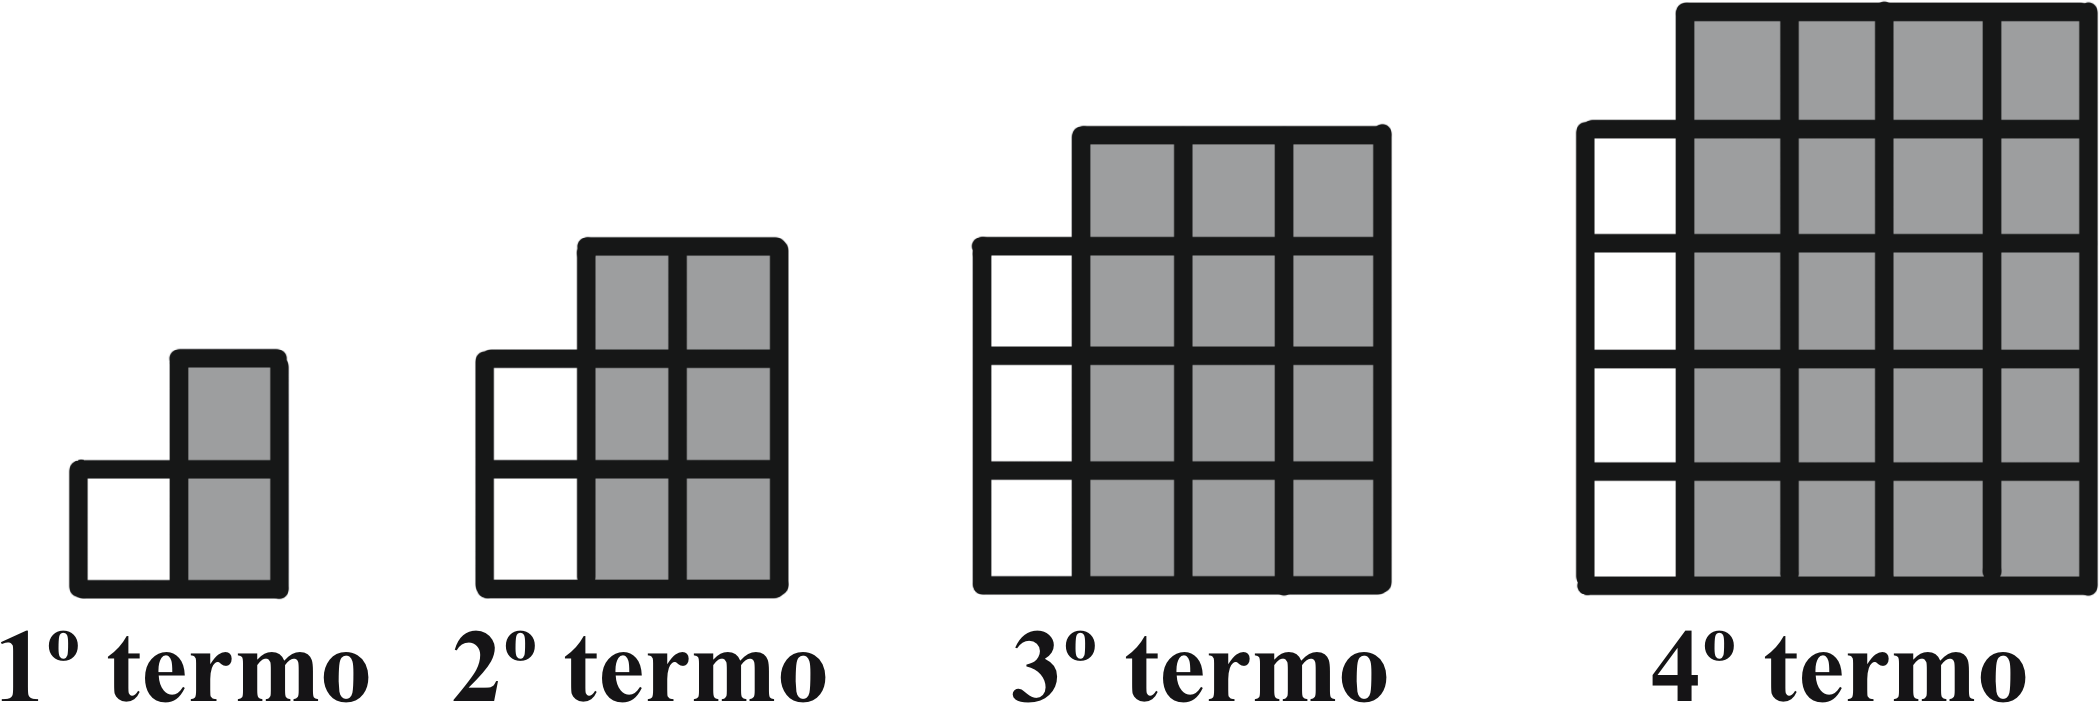
\includegraphics[width=\textwidth]{./ilustras-mat/Simulado_4-_atividade_6.png}
%\end{figure}

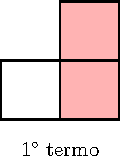
\includegraphics[page=1,scale=.85]{./tikz/048.pdf}\quad
\includegraphics[page=2,scale=.85]{./tikz/048.pdf}\quad
\includegraphics[page=3,scale=.85]{./tikz/048.pdf}\quad
\includegraphics[page=4,scale=.85]{./tikz/048.pdf}

Ficou perceptível que a quantidade de azulejos pintados era dada pela
seguinte expressão q = n \cdot (n + 1), sendo \textbf{n} o número do termo e
\textbf{q} a quantidade de azulejos. Qual será a quantidade de azulejos
pintados no 8º termo?

\begin{multicols}{2}
\begin{escolha}

\item
  44
\item
  49
\item
  56
\item
  72
\end{escolha}
\end{multicols}

\pagebreak
\num{7} A expressão determina o número total de diagonais de um polígono convexo, em que D representa o número total de diagonais do polígono, e \emph{n} o número de lados. 

Qual é o número de lados de um polígono que tem 14 diagonais?

\begin{escolha}
\item 35

\item 32

\item 10

\item 7
\end{escolha}



\num{8} Uma das grandes preocupações de hoje é a quantidade de açúcar ingerido, por isso as pessoas têm ficado mais atentar aos dados da embalagem.

Em uma embalagem de um chocolate, consta que, em cada 100 gramas de
chocolate, contém 24 gramas de açúcar. Fernando comprou uma barra de 450
gramas desse chocolate.

Quantos gramas de açúcar contém essa barra que Fernando comprou?

\begin{escolha}
\item 48 

\item 96 

\item 108 

\item 160
\end{escolha}

\num{9} Avaliando o consumo de bolas de sorvete e a temperatura foi anotado
os dados na tabela:

\begin{longtable}[]{@{}llllllll@{}}
\toprule\noalign{}
\emph{temperatura média mensal (ºC)} & \textbf{23} & \textbf{24} &
\textbf{25} & \textbf{27} & \textbf{28} & \textbf{29} & \textbf{30} \\
\midrule\noalign{}
\endhead
\bottomrule\noalign{}
\endlastfoot
\emph{bolas de sorvete} & 860 & 880 & 900 & 940 & 960 & 980 & 1000 \\
\end{longtable}

A regularidade se mantendo, qual seria a quantidade de bolas de sorvete
em um dia de temperatura de 34 º

\begin{escolha}
\item 1010

\item 1020

\item 1040

\item 1060
\end{escolha}


\pagebreak
\num{10} Observe a figura.

\begin{figure}[htpb!]
\centering
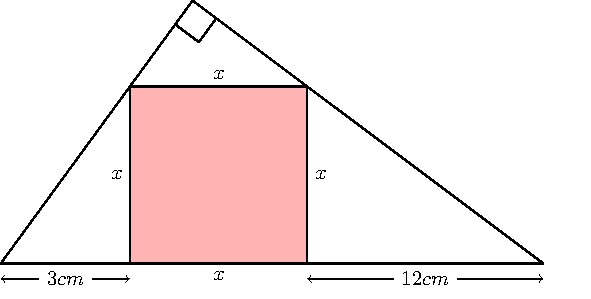
\includegraphics[width=.5\textwidth]{./tikz/049.pdf}
\end{figure}

Qual a medida do lado do quadrado?

\begin{multicols}{2}
\begin{escolha}
\item 10.

\item 8.

\item 6.

\item 4.
\end{escolha}
\end{multicols}

\num{11} Numa pesquisa de opinião, feita para verificar o nível de aprovação
de um produto, foram entrevistadas 1000 pessoas, que responderam sobre a
qualidade de uma marca de sabão em pó, escolhendo-se apenas uma
resposta.

O gráfico abaixo mostra o resultado da pesquisa.

\begin{figure}[htpb!]
\centering
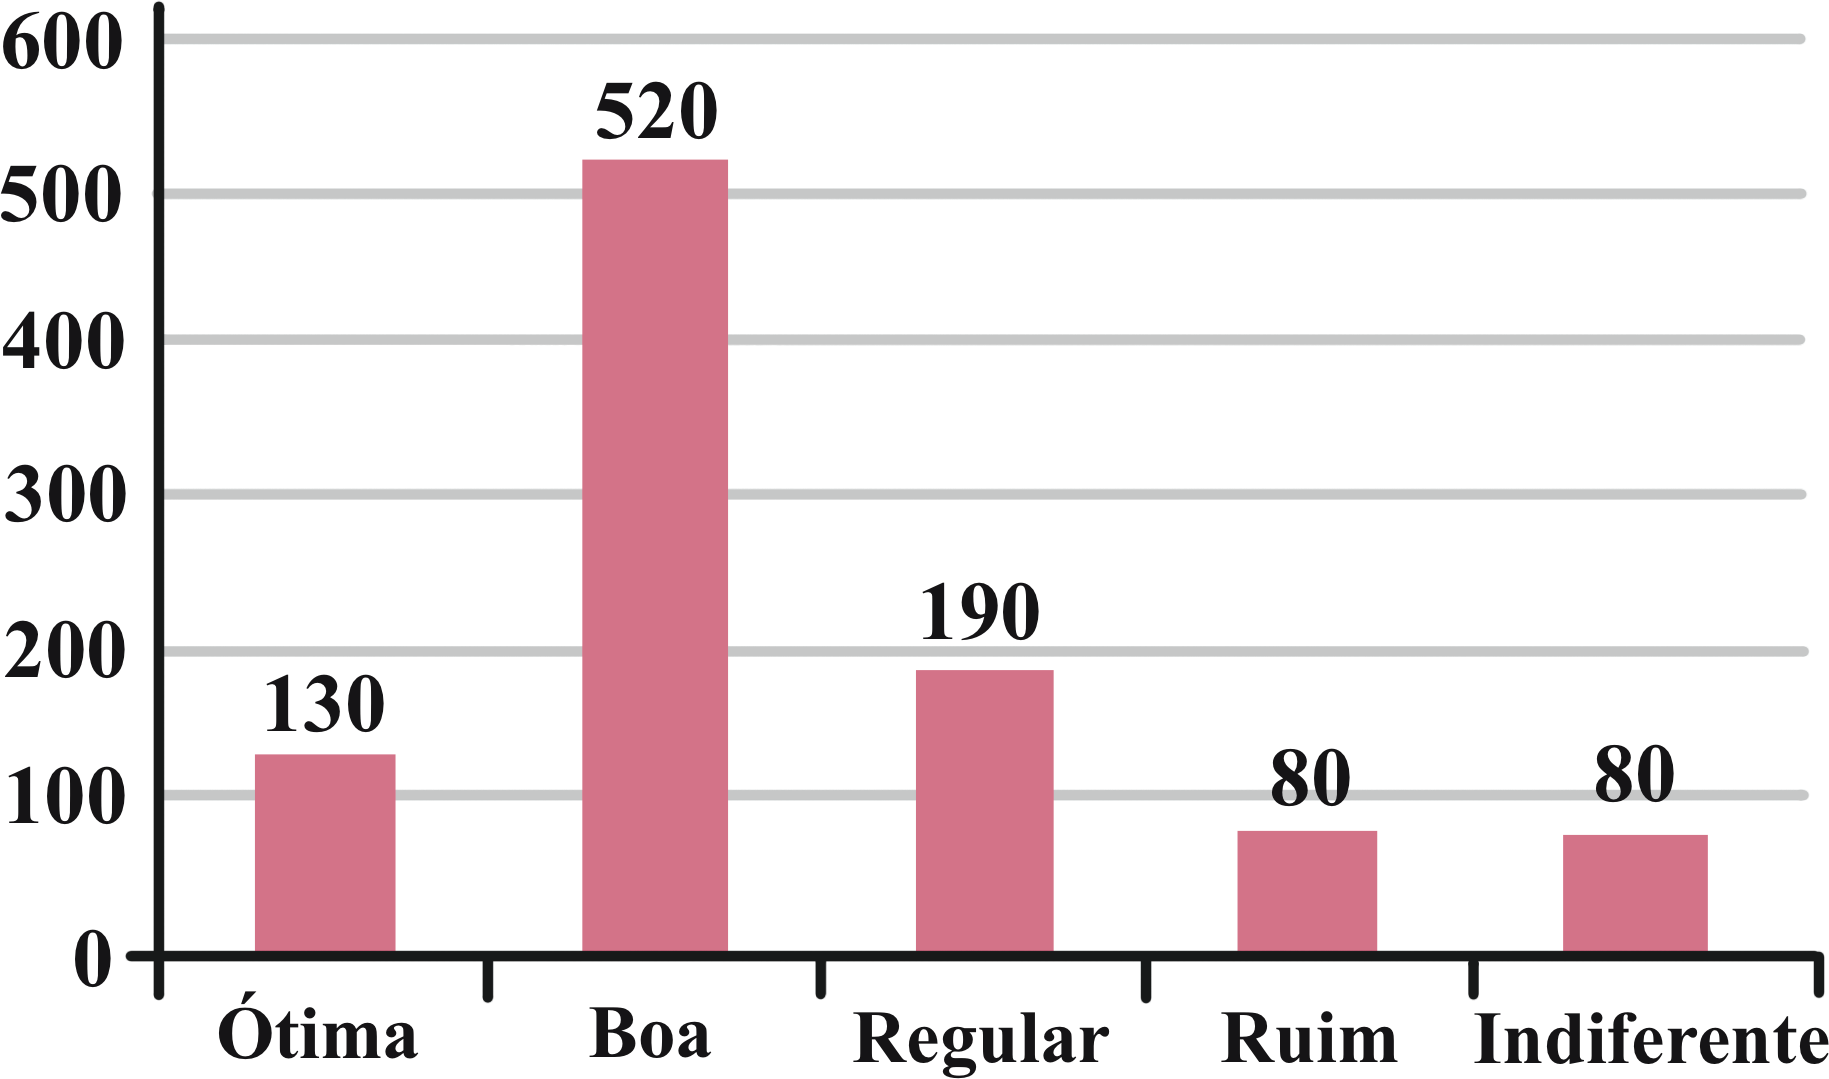
\includegraphics[width=.75\textwidth]{./ilustras-mat/Simulado_4-atividade_11.png}
\end{figure}

%Refazer o gráfico

De acordo com o gráfico, pode-se afirmar que o percentual de pessoas que
consideram a marca de sabão em pó boa ou regular é de:

\begin{multicols}{2}
\begin{escolha}
\item 28\%.

\item 65\%.

\item 71\%.

\item 84\%.
\end{escolha}
\end{multicols}

\pagebreak
\num{12} Uma empresa está analisando se coloca seu produto em um tipo de
cilindro de 6 cm de raio ou em um mais alto com 3 cm de raio.

\begin{figure}[htpb!]
\centering
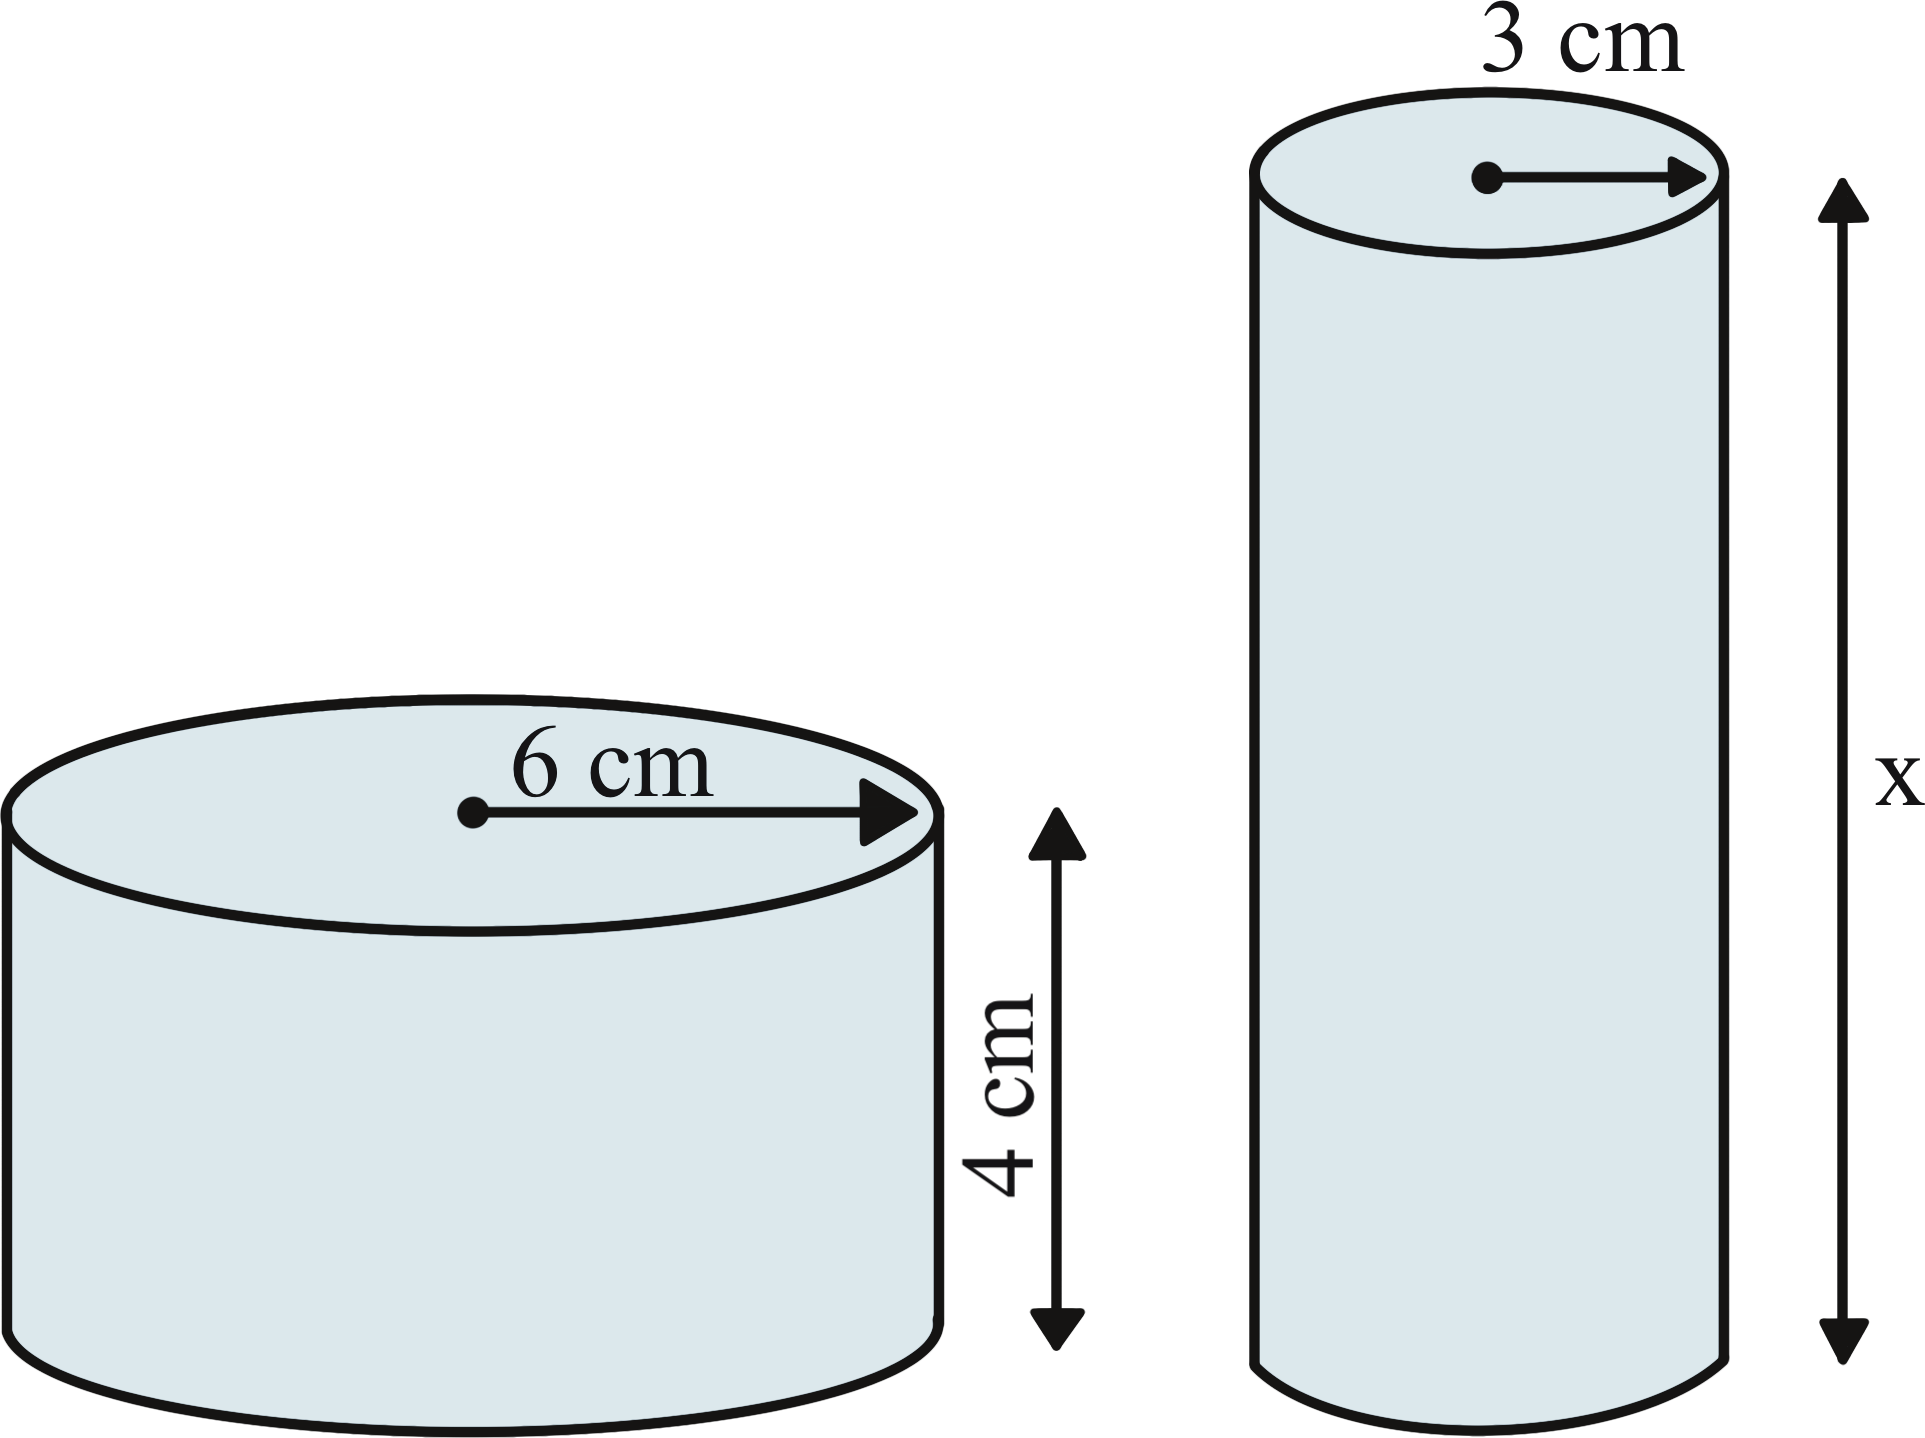
\includegraphics[width=\textwidth]{./ilustras-mat/Simulado_4-atividade_12.png}
\end{figure}

Sabendo que os volumes são iguais, qual o valor de x?

\begin{escolha}
\item
  8
\item
  12
\item
  16
\item
  20
\end{escolha}

\num{13} As notas de um grupo de alunos em suas provas de Matemática foram:
8,4; 9,1; 7,2; 6,8; 8,7 e 7,2.

Qual a média e a mediana respectivamente?

\begin{multicols}{2}
\begin{escolha}
\item 7,9; 7,8

\item 7,2; 7,8

\item 7,8; 7,8

\item 7,8; 7,9
\end{escolha}
\end{multicols}

\num{14} Um reservatório é formado por uma caixa de forma cúbica com 1 metro
de lado e está acoplada a um cano cilíndrico com 4 cm de diâmetro e 50 m
de comprimento.

Qual o volume total do sistema quando está completamente cheio?

\begin{escolha}
\item 1 000 litros.

\item 1015 litros.

\item 1 062,8 litros.

\item 1600 litros.
\end{escolha}


\num{15} O dominó é um jogo de tabuleiro que tem origem incerta, mas é
geralmente associado aos países europeus e latino-americanos. Há várias
teorias sobre a sua origem, mas nenhuma delas é totalmente comprovada.

Uma das teorias é que o dominó teria sido criado na China, por volta do
século XII, durante a Dinastia Song. No entanto, essa teoria é
controversa e não há evidências históricas que comprovem a sua
veracidade.

Outra teoria é que o dominó teria sido criado na Europa, mais
precisamente na Itália ou na França, durante o século XVIII. Nessa
época, o jogo era conhecido como "dominoes" e era jogado com peças de
madeira.

Independentemente da sua origem, o dominó se tornou um jogo muito
popular em todo o mundo, especialmente em países como México, Brasil e
Cuba, onde é considerado um símbolo da cultura local.

\begin{figure}[htpb!]
\centering
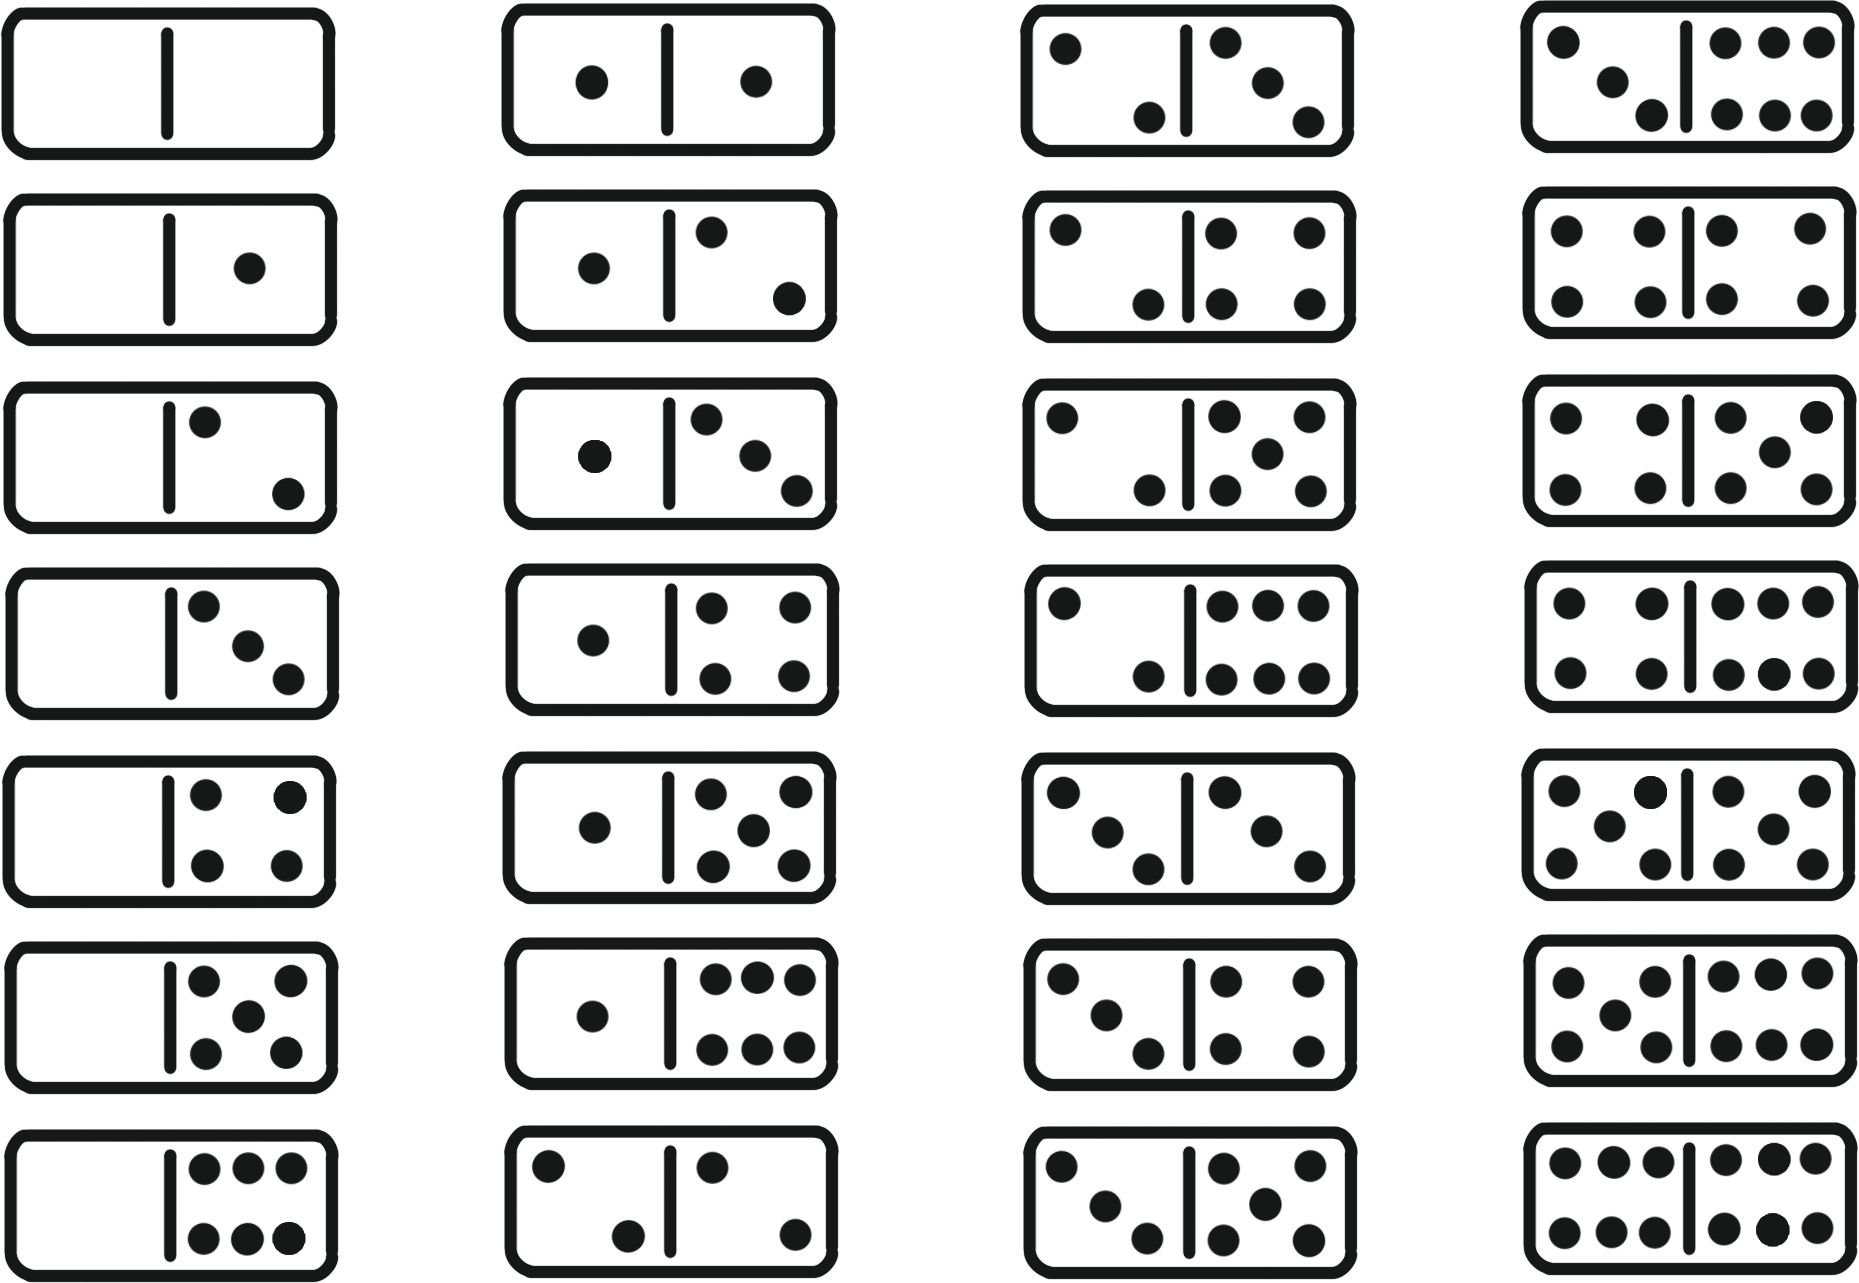
\includegraphics[width=\textwidth]{./ilustras-mat/Simulado_4-atividade_15.png}
\end{figure}

%Procurar outra imagem para ilustrar

Qual a probabilidade de ao escolher uma peça ao acaso e ela tenha dois
números diferentes entre si?

\begin{escolha}

\item
  25\%.
\item
  75\%.
\item
  35\%.
\item
  60\%.
\end{escolha}


\num{16} Leia o texto a seguir:

\begin{quote}
A atividade física é importante para o pleno desenvolvimento humano e
deve ser praticada em todas as fases da vida e em diversos momentos.
Além de apresentar inúmeros benefícios para a proteção e prevenção de
Doenças Crônicas Não Transmissíveis (DCNTs), a prática também tem
influência positiva nos aspectos psicológicos e sociais. Isso porque
muitas atividades coletivas incentivam a socialização, sendo esse um
elemento importante para todos, principalmente para crianças e
adolescentes, como parte da formação, assim como é um poderoso estímulo
para pessoas idosas.

\fonte{Ministério da Saúde. Conheça o primeiro Guia de Atividade Física para a População Brasileira. Disponível em:
https://www.gov.br/saude/pt-br/assuntos/saude-brasil/eu-quero-me-exercitar/noticias/2021/conheca-o-primeiro-guia-de-atividade-fisica-para-a-populacao-brasileira.
Acesso em: 22 fev. 2023.}
\end{quote}

Considerando as afirmações do texto, é possível afirmar que as atividades
físicas

\begin{escolha}
\item devem restringir-se a crianças, jovens e idosos.

\item agravam ocorrências de Doenças Crônicas Não Transmissíveis.

\item beneficiam não apenas as pessoas, mas também a sociedade.

\item impactam a saúde física, sem efeitos psicológicos.
\end{escolha}

\num{17}  Leia a reportagem a seguir:

\begin{quote}
Iniciam amanhã, os Jogos Escolares Eletrônicos do Paraná. A 2ª edição da
competição acontecerá em 5 finais de semana nos meses de setembro e
outubro. A introdução do \textit{e-sports} nos Jogos Oficiais do Estado aconteceu
ano passado visando o intercâmbio e o entretenimento, aproximando os
alunos, como forma de atenuar os efeitos nocivos causados pela pandemia
da Covid-19.~{[}...{]}

Para a coordenadora dos Jogos Escolares do Paraná, Márcia Tomadon,
``tomamos esta medida para que todos os alunos possam participar. Muitas
vezes as escolas não conseguem montar uma equipe, então desta maneira
damos a possibilidade de todos estarem contemplados na competição, e
assim também já conseguimos uma interação entre crianças de escolas
diferentes''. Ela também ressaltou o bom número de alunos inscritos:
``foram 2.742 inscrições, um bom número tendo em vista que estamos
introduzindo o \textit{e-sports} na cultura esportiva escolar''.

\fonte{Paraná Esporte. Jogos Escolares Eletrônicos tem início neste sábado. 
Disponível em:
https://www.esporte.pr.gov.br/Noticia/Jogos-Escolares-Eletronicos-tem-inicio-neste-sabado.
Acesso em: 12 abr. 2023.}
\end{quote}

\pagebreak
Considerando as informações apresnetadas na reportagem, é possível afirmar
que os \textit{e-sports}

\begin{escolha}
\item contribuíram para a integração dos alunos durante a pandemia.

\item estão passando pelo processo de se tornarem esporte oficial.  

\item causaram efeitos nocivos durante a pandemia.

\item reduziram a integração entre alunos de diferentes escolas.
\end{escolha}

\num{18}  Leia o texto a seguir:

\begin{quote}
Apesar de adorar dançar, Mara Raymundo começou a dançar como forma de
exercício físico para melhorar picos de pressão que tinha por conta da
vida agitada. ``Não queria tomar remédio, então fui dançar e hoje tenho a
pressão normal'', justifica Mara. Mas não foi só a pressão da Mara que
melhorou. ``A memória melhorou, decorando os passos da dança, e a relação
com os outros também, além do humor, do sono e da disposição. Me sinto
como se tivesse 15 anos'', comemora. Há um ano e meio ela dança duas
horas por dia, três vezes na semana, e ainda sai para dançar com os
amigos nos fins de semana. ``A música eleva, inspira'', completa.

\fonte{Ministério da Saúde. Dançar faz bem ao corpo, à alma e à mente. 
Disponível em:
https://www.gov.br/saude/pt-br/assuntos/saude-brasil/eu-quero-me-exercitar/noticias/2018/dancar-faz-bem-ao-corpo-a-alma-e-a-mente.
Acesso em: 12 abr. 2023.}
\end{quote}

Considerando as afirmações da reportagem, é possível afirmar que os 
benefícios da dança  

\begin{escolha}
\item estão condicionados ao uso de remédios prescritos.

\item levaram Mara ao desfrute da arte e à reclusão social.

\item impactaram a saúde física, mental e emocional de Mara.

\item revelaram que os problemas de pressão não eram reais.
\end{escolha}


\num{19}
\begin{quote}
  Fusão nuclear e fissão nuclear são diferentes. A fissão é usada desde 1950 nos reatores de energia
  atômica. Na fusão a energia é gerada a partir da união de átomos; na fissão a energia é gerada pela divisão de átomos. A fusão
  é o processo que ocorre no Sol continuamente, responsável por seu
  calor e por sua luz.

\fonte{Fonte de pesquisa: Matt McGrath. BBC News Brasil. O que é a fusão nuclear, que promete ser a energia limpa que o mundo procura. Disponível em:
https://www.bbc.com/portuguese/geral-50422745. Acesso em: 25 fev. 2023.}
\end{quote}

\pagebreak
Com base nos materiais e no processo utilizados para a produção de
energia a partir da fusão nuclear, podemos afirmar que

\begin{escolha}
\item
  Trata-se da união de elétrons a partir de liberação uma grande quantidade de energia.
\item
  Trata-se da união de dois núcleos, para formar um mais denso, sendo
  necessária grande quantidade de energia e pressão.
\item
  Trata-se de um processo prejudicial que gera lixo radioativo, pois
  utiliza compostos químicos tóxicos.
\item
  Trata-se de um processo barato e simples, já que se trata de uma cópia
  de um processo que ocorre naturalmente no Sol.
\end{escolha}

\num{20}
\begin{quote}
  De acordo com sua teoria, há uma luta pela sobrevivência na
  natureza, mas aquele que sobrevive não é necessariamente o mais forte
  e, sim, o que melhor se adapta às condições do ambiente em que vive.
  No ambiente árido, as tartarugas de pescoço longo alcançavam os
  arbustos para se alimentar. Enquanto aquelas que viviam em local
  úmido, podiam comer grama e se proteger dos predadores graças ao
  pescoço curto e à carapaça arredondada.

\fonte{BBC News Brasil. O que é a teoria da evolução de Charles Darwin e o que inspirou suas ideias revolucionárias. Disponível em:
https://www.bbc.com/portuguese/geral-50525124. Acesso em: 23 fev. 2023.}
\end{quote}

A partir do texto e de seus conhecimentos, identifique a alternativa que
apresenta o conceito e o cientista por trás do conceito descrito.

\begin{escolha}
\item
  Lei do uso e desuso, Darwin.
\item
  Lei dos caracteres adquiridos, Lamarck.
\item
  Lei da seleção natural, Darwin.
\item
  Lei da seleção natural, Lamarck.
\end{escolha}

\num{21}
  \begin{quote}
 \emph{Mars One} é um projeto holendês lançado em 2012. Foram
  escolhidas quarenta pessoas, entre 200 mil candidatos. O projeto, 
  financiado por um programa estilo "reality show", tem como objetivo proporcionar um treinamento de sobrevivência em Marte. Há quem considere o projeto uma brincadeira, mas também há quems e interesse muito pelo assunto. A empresa \emph{SpaceX} também tem projetos (um pouco mais sérios)
  para Marte. A empresa
  imagina um veículo gigante usado para promover o  entre a Terra e Marte.

\fonte{Fonte de pesquisa: BBC News Brasil. Disponível em:
https://www.bbc.com/portuguese/noticias/2014/10/141010\_vert\_fut\_colonia\_espaco\_dg.
Acesso em: 25 fev. 2023.}
\end{quote}

\pagebreak
Imaginando que a colonização espacial seja uma realidade próxima, quais seriam
possíveis consequências para o corpo de seres humanos nascidos no espaço?

\begin{escolha}
\item
  Os corpos se tornam mais altos devido à ausência de gravidade e a
  diminuição do volume de sangue, já que há menos esforço para o coração.
\item
  Pelo maior contato com a radiação, os seres humanos seriam mais
  tolerantes a desenvolver câncer.
\item
  Haveria o aumento da massa muscular e óssea provocadas pela
  microgravidade espacial, porém uma diminuição na altura.
\item
  Melhora nas condições da visão devido ao controle de exposição a luz,
  acompanhadas de insônia pela diferença no fuso.
\end{escolha}




